\documentclass[preprint,12pt,aps,pra,showkeys,amsmath,amssymb,superscriptaddress,floatfix]{revtex4-2}
\usepackage[T1]{fontenc}
\usepackage[utf8]{inputenc}
\usepackage{amsmath,amssymb,amsthm,mathtools,mathrsfs}
\usepackage{microtype,booktabs,enumitem}
\usepackage{xcolor,tikz,etoolbox}
\usepackage[skins,breakable]{tcolorbox}
\usepackage{needspace}
% Keep diagram geometry independent of REVTeX preprint body spacing.
\AtBeginEnvironment{tikzpicture}{\linespread{1}\selectfont}
\usetikzlibrary{arrows.meta,positioning,calc,fit,decorations.pathreplacing}
\usepackage{graphicx}
\usepackage{hyperref}

\definecolor{MMBlue}{RGB}{0,82,155}
\definecolor{MMOrange}{RGB}{200,80,0}
\tikzset{
 mmnode/.style={draw=MMBlue,rounded corners=2pt,fill=MMBlue!4,align=left,execute at begin node={\raggedright},text width=5cm,font=\fontsize{10}{12}\selectfont,inner sep=6pt},
 mmimport/.style={mmnode,draw=black!65,fill=black!4},
 mmcandidate/.style={mmnode,draw=MMOrange,dashed,fill=MMOrange!5},
 mmrejected/.style={mmnode,draw=black,densely dotted,fill=black!8},
 mmproof/.style={->,thick,MMBlue},
 mmflow/.style={->,semithick,black!70},
 mmrepair/.style={->,dashed,thick,MMOrange},
 mmcandidatearrow/.style={->,dashed,semithick,MMOrange},
 mmnote/.style={font=\scriptsize,fill=white,inner sep=2pt,align=center}}

\usepackage[section]{placeins}
\setlength{\emergencystretch}{3em}
\setlist{itemsep=3pt,topsep=4pt}
\newtheorem{theorem}{Theorem}[section]
\newtheorem{proposition}[theorem]{Proposition}
\newtheorem{lemma}[theorem]{Lemma}
\newtheorem{corollary}[theorem]{Corollary}
\theoremstyle{definition}
\newtheorem{definition}[theorem]{Definition}
\newtheorem{example}[theorem]{Example}
\theoremstyle{remark}
\newtheorem{remark}[theorem]{Remark}
% Avoid isolated statement headings and single-line paragraph fragments.
\BeforeBeginEnvironment{theorem}{\Needspace{6\baselineskip}}
\BeforeBeginEnvironment{definition}{\Needspace{5\baselineskip}}
\BeforeBeginEnvironment{proposition}{\Needspace{5\baselineskip}}
\BeforeBeginEnvironment{lemma}{\Needspace{5\baselineskip}}
\BeforeBeginEnvironment{corollary}{\Needspace{5\baselineskip}}
\clubpenalty=5000
\widowpenalty=5000
\newcommand{\R}{\mathbb R}\newcommand{\Z}{\mathbb Z}\newcommand{\N}{\mathbb N}
\newcommand{\Pa}{\operatorname{Pa}}\newcommand{\Desc}{\operatorname{Desc}}
\newcommand{\cl}{\operatorname{cl}}\newcommand{\cost}{\operatorname{cost}}
\newcommand{\status}{\operatorname{status}}
% Faculty cards: a visual rail groups the five faculties within one agent.
% The rail has no arrowhead and does not represent a proof dependency.
\newcommand{\mmfacultybadge}[1]{%
 \node[circle,draw=MMBlue,line width=1pt,fill=white,
 minimum size=7mm,inner sep=0pt,font=\sffamily\small\bfseries,text=MMBlue]
 at ([xshift=15pt,yshift=-15pt]frame.north west) {#1};}
\newcommand{\mmfacultyrail}{%
 \draw[MMBlue!80,line width=1pt]
 ([xshift=15pt,yshift=2pt]frame.north west)--
 ([xshift=15pt,yshift=-2pt]frame.south west);}
\newtcolorbox{mmfacultybox}[2]{enhanced,breakable,
 colback=MMBlue!4,colframe=MMBlue!4,boxrule=0pt,arc=3pt,
 left=39pt,right=9pt,top=4pt,bottom=4pt,
 before skip=2pt,after skip=2pt,
 fontupper=\small\linespread{1.1}\selectfont,
 overlay unbroken={\mmfacultyrail\mmfacultybadge{#1}},
 overlay first={\mmfacultyrail\mmfacultybadge{#1}},
 overlay middle={\mmfacultyrail},overlay last={\mmfacultyrail}}
\newcommand{\mmfaculty}[3]{%
 \begin{mmfacultybox}{#1}{#2}
 {\sffamily\bfseries\color{MMBlue}#2}\par\smallskip #3
 \end{mmfacultybox}}
\newcommand{\agent}[9]{%
 \Needspace{8\baselineskip}
 \subsubsection{#1}
 \noindent\textbf{Object.} #2\par
 \noindent\textbf{Role.} #3\par\smallskip
 \mmfaculty{E}{Ego}{#4}
 \mmfaculty{M}{Memory}{#5}
 \mmfaculty{I}{Intellect}{#6}
 \mmfaculty{S}{Sense}{#7}
 \mmfaculty{A}{Action}{#8}
 \smallskip\noindent #9\par}

\usepackage{longtable,array,calc}
\providecommand{\tightlist}{\setlength{\itemsep}{2pt}\setlength{\parskip}{0pt}}
\makeatletter
\def\frontmatter@abstract@produce{\par\addvspace{\frontmatter@preabstractspace}%
\begingroup\prep@absbox\unvbox\absbox\post@absbox\endgroup
\addvspace{\frontmatter@postabstractspace}}
\makeatother
\newcommand{\field}[2]{\par\smallskip\noindent\textbf{#1.} #2\par}
\setlength{\emergencystretch}{5em}
\AtBeginEnvironment{verbatim}{\small\linespread{1.0}\selectfont}


\hypersetup{colorlinks=true,linkcolor=MMBlue,urlcolor=MMBlue,pdfauthor={Dibakar Sigdel}}

\begin{document}

\title{Singular Value Decomposition\\[4pt]\large An End-to-End Meta-Math Walkthrough}

\author{Dibakar Sigdel}

\affiliation{Mindverse Computing LLC, Lynnwood, WA 98087, USA}

\date{October 2026}

\begin{abstract}

A complete authored walkthrough of singular value decomposition, with
explicit mathematical contracts, local verification gates, and reusable
exports. The report presents the target theorem, declared imports, a
dependency graph, five-faculty node contracts, a continuous proof, a
worked example, and a hypothesis-repair audit. It is an authored
mathematical exposition, not a deployed-agent transcript or a formal
proof-assistant certificate.

\end{abstract}\maketitle\linespread{1.12}\selectfont

\noindent\textbf{LA-04 / Linear Algebra / Report v1}

\section{Target and import contract}

\begin{theorem}

For every real \(m\times n\) matrix \(A\), prove \(A=U\Sigma V^T\) with
orthogonal \(U,V\) and rectangular diagonal \(\Sigma\) having
nonnegative singular values.

\end{theorem}

\subsection{Foundations and permitted imports}

Import LA-03: every real symmetric matrix has an orthonormal eigenbasis.
Import orthonormal completion from LA-02 and LA-01's finite-dimensional
kernel/rank facts. For \(A:R^{n}\to R^{m}\), the matrix \(A^{T}A\) is
symmetric positive semidefinite. U and V are square orthogonal matrices;
\(\Sigma\) is \(m\times n\) with nonnegative entries on its rectangular
diagonal.

\clearpage\section{Node interaction workflow}

\begin{center}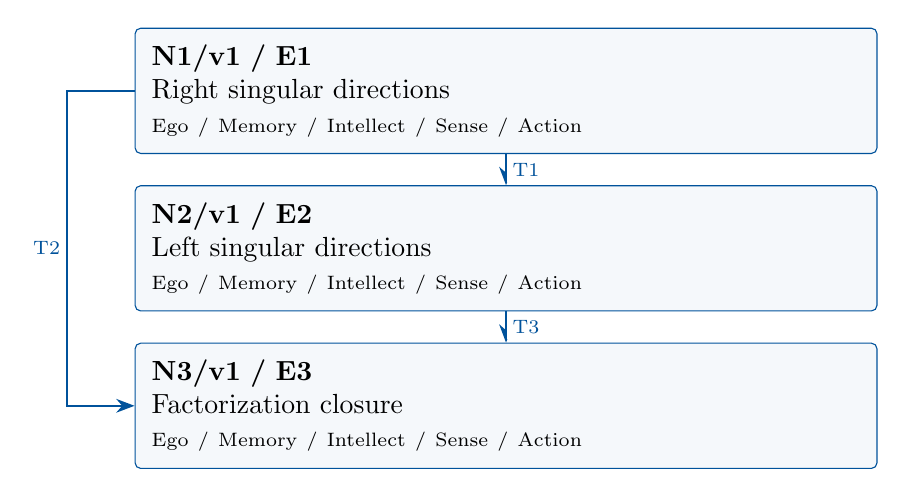
\begin{tikzpicture}[>=Stealth,x=1cm,y=1cm]

\node[mmnode,text width=9cm,minimum height=1.25cm] (N1) at (0,0.0) {\textbf{N1/v1 / E1}\\Right singular directions\\{\scriptsize Ego / Memory / Intellect / Sense / Action}};

\node[mmnode,text width=9cm,minimum height=1.25cm] (N2) at (0,-2.0) {\textbf{N2/v1 / E2}\\Left singular directions\\{\scriptsize Ego / Memory / Intellect / Sense / Action}};

\node[mmnode,text width=9cm,minimum height=1.25cm] (N3) at (0,-4.0) {\textbf{N3/v1 / E3}\\Factorization closure\\{\scriptsize Ego / Memory / Intellect / Sense / Action}};

\draw[mmproof] (N1.south) -- node[mmnote,right] {T1} (N2.north);

\draw[mmproof] (N1.west) -- (-5.58,0) -- node[mmnote,left] {T2} (-5.58,-4) -- (N3.west);

\draw[mmproof] (N2.south) -- node[mmnote,right] {T3} (N3.north);

\end{tikzpicture}\end{center}

Each box is one mathematical agent containing all five faculties. Blue
arrows carry the versioned exports listed below. The layout gives a
reading order; only drawn arrows assert dependencies. Diagnostic repair
is separate from the proof DAG.

\subsection{Versioned evidence-transfer ledger}

\begingroup\small\linespread{1.05}\selectfont

\Needspace{5\baselineskip}\field{T1: N1/E1/v1 to N2}{An orthonormal right basis with \(Av_i=0\) for \(i>r\).}

\field{Receiving activity}{N2: Left singular directions}

\field{Compatibility}{Use the same mathematical objects and hypotheses as the source export.
Receiving contract: Positive \(\sigma _i\) and right eigenvectors; prior
exports E1/v1}

\Needspace{5\baselineskip}\field{T2: N1/E1/v1 to N3}{An orthonormal right basis with \(Av_i=0\) for \(i>r\).}

\field{Receiving activity}{N3: Factorization closure}

\field{Compatibility}{Use the same mathematical objects and hypotheses as the source export.
Receiving contract: Both orthonormal bases; prior exports E1/v1, E2/v1}

\Needspace{5\baselineskip}\field{T3: N2/E2/v1 to N3}{A full orthonormal left basis whose first r vectors match positive
singular directions.}

\field{Receiving activity}{N3: Factorization closure}

\field{Compatibility}{Use the same mathematical objects and hypotheses as the source export.
Receiving contract: Both orthonormal bases; prior exports E1/v1, E2/v1}

\endgroup

\clearpage\section{Agent roles and five-faculty activities}\begingroup\small\linespread{1.05}\selectfont\setlist{itemsep=1pt,topsep=2pt}

\subsection{N1/v1: Right singular directions}

\field{Object and role}{Order positive eigenvalues before zero ones.}

\field{Inputs}{Spectral theorem on \(A^{T}A\); foundational imports stated in §1}

\mmfaculty{E}{Ego}{Own E1/v1: An orthonormal right basis with \(Av_i=0\) for \(i>r\).}

\mmfaculty{M}{Memory}{Retain Spectral theorem on \(A^{T}A\); foundational imports stated in
§1; keep their assumptions and versions attached.}

\mmfaculty{I}{Intellect}{Order positive eigenvalues before zero ones.}

\mmfaculty{S}{Sense}{Negative eigenvalues cannot occur; tiny computed negatives are numerical
errors, not theorem data.}

\mmfaculty{A}{Action}{Carry out the numbered deductions and publish E1/v1 together with its
hypotheses and proof location.}

\smallskip\noindent\textbf{Numbered mathematical activities}

\begin{enumerate}[label=N1.\arabic*,leftmargin=3.4em]

\item Let \(v_{1},\ldots ,v_n\) be an orthonormal eigenbasis of \(A^{T}A\)
with eigenvalues \(\lambda _i\).

\item Since \(v_i^{T}A^{T}Av_i=\Vert Av_i\Vert ^{2}\ge 0\), all
\(\lambda _i\ge 0\).

\item Arrange \(\lambda _{1},\ldots ,\lambda _r>0\) and the rest zero; put
\(\sigma _i=\sqrt{\lambda _i}\).

\item For \(\lambda _i=0\), \(\Vert Av_i\Vert ^{2}=0\), so \(Av_i=0\).

\item Moreover \(\operatorname{ker} (A^{T}A)=\operatorname{ker} A\) by this
same norm identity, so \(r=\operatorname{rank} A\).

\end{enumerate}

\field{Export E1/v1}{An orthonormal right basis with \(Av_i=0\) for \(i>r\).}

\field{Acceptance gate}{Negative eigenvalues cannot occur; tiny computed negatives are numerical
errors, not theorem data. Publish only after checking every displayed
deduction.}

\field{Targeted repair}{If the check fails, revise N1: Negative eigenvalues cannot occur; tiny
computed negatives are numerical errors, not theorem data. Recheck
dependent nodes N2, N3.}

\clearpage

\subsection{N2/v1: Left singular directions}

\field{Object and role}{Normalize only nonzero images.}

\field{Inputs}{Positive \(\sigma _i\) and right eigenvectors; prior exports E1/v1}

\mmfaculty{E}{Ego}{Own E2/v1: A full orthonormal left basis whose first r vectors match
positive singular directions.}

\mmfaculty{M}{Memory}{Retain Positive \(\sigma _i\) and right eigenvectors; prior exports
E1/v1; keep their assumptions and versions attached.}

\mmfaculty{I}{Intellect}{Normalize only nonzero images.}

\mmfaculty{S}{Sense}{The zero singular values require completion, not normalization.}

\mmfaculty{A}{Action}{Carry out the numbered deductions and publish E2/v1 together with its
hypotheses and proof location.}

\smallskip\noindent\textbf{Numbered mathematical activities}

\begin{enumerate}[label=N2.\arabic*,leftmargin=3.4em]

\item For \(i\le r\) define \(u_i=Av_i/\sigma _i\).

\item Then
\(u_i^{T}u_j=v_i^{T}A^{T}Av_j/(\sigma _i\sigma _j)=\lambda _j\delta _{ij}/(\sigma _i\sigma _j)=\delta _{ij}\).

\item Thus these r vectors are orthonormal in \(R^{m}\), in particular
\(r\le m\).

\item Complete them to an orthonormal basis \(u_{1},\ldots ,u_m\) without
attempting to divide zero images by zero singular values.

\end{enumerate}

\field{Export E2/v1}{A full orthonormal left basis whose first r vectors match positive
singular directions.}

\field{Acceptance gate}{The zero singular values require completion, not normalization. Publish
only after checking every displayed deduction.}

\field{Targeted repair}{If the check fails, revise N2: The zero singular values require
completion, not normalization. Recheck dependent nodes N3.}

\clearpage

\subsection{N3/v1: Factorization closure}

\field{Object and role}{Check the equality on every basis vector.}

\field{Inputs}{Both orthonormal bases; prior exports E1/v1, E2/v1}

\mmfaculty{E}{Ego}{Own E3/v1: The full real rectangular SVD with nonnegative singular
values.}

\mmfaculty{M}{Memory}{Retain Both orthonormal bases; prior exports E1/v1, E2/v1; keep their
assumptions and versions attached.}

\mmfaculty{I}{Intellect}{Check the equality on every basis vector.}

\mmfaculty{S}{Sense}{No uniqueness of U or V is asserted.}

\mmfaculty{A}{Action}{Carry out the numbered deductions and publish E3/v1 together with its
hypotheses and proof location.}

\smallskip\noindent\textbf{Numbered mathematical activities}

\begin{enumerate}[label=N3.\arabic*,leftmargin=3.4em]

\item Let V have columns \(v_i\), U have columns \(u_i\), and \(\Sigma\) have
\(\sigma _i\) at (i,i) for \(i\le r\) and zeros elsewhere.

\item For \(i\le r\), \(U\Sigma V^{T}v_i=\sigma _i\) \(u_i=Av_i\); for \(i>r\)
both sides vanish.

\item Since \(v_i\) form a basis, \(A=U\Sigma V^{T}\).

\item This includes \(A=0\) and rectangular dimensions.

\item The sorted singular values are determined by the eigenvalues of
\(A^{T}A\); bases in repeated or zero eigenspaces need not be unique.

\end{enumerate}

\field{Export E3/v1}{The full real rectangular SVD with nonnegative singular values.}

\field{Acceptance gate}{No uniqueness of U or V is asserted. Publish only after checking every
displayed deduction.}

\field{Targeted repair}{If the check fails, revise N3: No uniqueness of U or V is asserted.
Withhold this terminal result until its gate passes.}

\endgroup\clearpage\section{Continuous mathematical proof}\label{sec:proof}

Read these steps in order as one proof; the diagram is optional.
Numbered activities identify the specific constructions and deductions
owned by each node.

\subsection{§4.N1 --- Right singular
directions}\label{n1-right-singular-directions}

\begin{enumerate}
\def\labelenumi{\arabic{enumi}.}
\item
  Let \(v_{1},\ldots ,v_n\) be an orthonormal eigenbasis of \(A^{T}A\)
  with eigenvalues \(\lambda _i\).
\item
  Since \(v_i^{T}A^{T}Av_i=\Vert Av_i\Vert ^{2}\ge 0\), all
  \(\lambda _i\ge 0\).
\item
  Arrange \(\lambda _{1},\ldots ,\lambda _r>0\) and the rest zero; put
  \(\sigma _i=\sqrt{\lambda _i}\).
\item
  For \(\lambda _i=0\), \(\Vert Av_i\Vert ^{2}=0\), so \(Av_i=0\).
\item
  Moreover \(\operatorname{ker} (A^{T}A)=\operatorname{ker} A\) by this
  same norm identity, so \(r=\operatorname{rank} A\).
\end{enumerate}

\subsection{§4.N2 --- Left singular
directions}\label{n2-left-singular-directions}

\begin{enumerate}
\def\labelenumi{\arabic{enumi}.}
\item
  For \(i\le r\) define \(u_i=Av_i/\sigma _i\).
\item
  Then
  \(u_i^{T}u_j=v_i^{T}A^{T}Av_j/(\sigma _i\sigma _j)=\lambda _j\delta _{ij}/(\sigma _i\sigma _j)=\delta _{ij}\).
\item
  Thus these r vectors are orthonormal in \(R^{m}\), in particular
  \(r\le m\).
\item
  Complete them to an orthonormal basis \(u_{1},\ldots ,u_m\) without
  attempting to divide zero images by zero singular values.
\end{enumerate}

\subsection{§4.N3 --- Factorization
closure}\label{n3-factorization-closure}

\begin{enumerate}
\def\labelenumi{\arabic{enumi}.}
\item
  Let V have columns \(v_i\), U have columns \(u_i\), and \(\Sigma\)
  have \(\sigma _i\) at (i,i) for \(i\le r\) and zeros elsewhere.
\item
  For \(i\le r\), \(U\Sigma V^{T}v_i=\sigma _i\) \(u_i=Av_i\); for
  \(i>r\) both sides vanish.
\item
  Since \(v_i\) form a basis, \(A=U\Sigma V^{T}\).
\item
  This includes \(A=0\) and rectangular dimensions.
\item
  The sorted singular values are determined by the eigenvalues of
  \(A^{T}A\); bases in repeated or zero eigenspaces need not be unique.
\end{enumerate}

\hfill$\square$

\section{Worked orchestration}

For \(A=[[3,0],[0,0],[0,0]]\), take \(V=I_{2},U=I_{3}\) and
\(\Sigma =A\). The singular values are 3 and 0; only the first left
vector comes from normalizing \(Av_{1}\). The other two are an
orthonormal completion.

\subsection{Boundary and hypothesis audit}

Trying \(u_i=Av_i/\sigma _i\) at \(\sigma _i=0\) is undefined even for
the zero matrix. Sense returns that boundary test; Memory supplies the
kernel identity, and Action completes an orthonormal basis for the
remaining directions.

\section{Illustrative failure and repair}

The following is an authored diagnostic scenario. Changed assumptions
define a new contract; they do not retroactively prove the original
statement.

\subsection{Failure and correction}
This is an authored teaching trace, not a recorded agent run.

\begin{enumerate}
\def\labelenumi{\arabic{enumi}.}
\tightlist
\item
  \textbf{Ego \(\to\) Memory:} register the §1 theorem, imports, and
  requested exports before beginning the proof.
\item
  \textbf{Intellect \(\to\) Action:} choose the bridges in §3 and carry
  out the numbered activities in §4; transmit only established E-exports
  along the §2 DAG.
\item
  \textbf{Sense \(\to\) responsible node:} test the specific
  boundary/failure in §5 and the node's individual audit. A failing
  candidate is withheld; downstream nodes may not use it.
\item
  \textbf{Memory + Intellect:} identify whether the error is an omitted
  condition, an invalid inference, or an attempted extension beyond the
  theorem. Restore the exact contract or explicitly state a different
  one.
\item
  \textbf{Action:} redo the affected mathematical activity using the
  repaired condition or inference. Recheck consuming nodes, rather than
  feeding their conclusions back as premises.
\item
  \textbf{Ego:} publish only the supported export with its assumptions
  and proof location. A hypothetical revised export is v2; the written
  proof here is the v1 exposition, not a claim that this repair was
  executed.
\end{enumerate}

\subsection{Hypothesis boundary}
Trying \(u_i=Av_i/\sigma _i\) at \(\sigma _i=0\) is undefined even for
the zero matrix. Sense returns that boundary test; Memory supplies the
kernel identity, and Action completes an orthonormal basis for the
remaining directions.

\subsection{Version and recheck}
Treat any changed assumption as a new contract. Recheck the revised
export and all of its descendants. A backward diagnostic never
establishes an earlier theorem. This is an authored teaching trace, not
an execution log.

\par\medskip\begingroup\small\linespread{1.0}\selectfont\noindent\textbf{Provenance.} This authored proof is complete relative to its declared imports. Reuse
each export with its assumptions, proof, and version. The original
Markdown remains available for comparison.
\par\endgroup

\end{document}
